\documentclass{article}
\usepackage[utf8]{inputenc}
\usepackage{amsmath}
\usepackage{graphicx}
\usepackage{wrapfig}
\usepackage{float}
\usepackage[format=plain, indention=0.5cm, aboveskip=0.1cm, belowskip=0cm]{caption}
\usepackage[paper=a4paper,left=35mm,right=35mm,top=35mm,bottom=35mm]{geometry}
\usepackage[english]{babel}
\usepackage{csvsimple}
\usepackage{array}
\usepackage{booktabs}
\usepackage{siunitx}
\usepackage{physics}
\usepackage{hyperref}
\usepackage[bottom]{footmisc}
\usepackage{textcomp}

\title{\huge Electrical conductivity of metals, semiconductors and superconductors}
\author{\Large Jonas Colve, Matrikelnr. 377593\\ \Large Anna Stollenwerk, Matrikelnr. 381103 \\Gruppe 43}
\date{26.03.2020}

\begin{document}
\renewcommand{\figurename}{fig.}
\renewcommand{\tablename}{tab.}

\maketitle
\newpage



\tableofcontents

\newpage

\section{Introduction}
The purpose of this experiment is to analyse the thermal dependence of the electrical conductivity in different materials.
The observed materials are copper, tantalum and silicon.\\
The electrical conductivity in solids with crystalline structure can be explained by Drude Theory, which claims that electrons behave like a free electron gas.
So the resistance is
\begin{equation*}
    \rho = \frac{m_{eff}}{n e^2\tau} = \frac{1}{\mu n e}
\end{equation*}
with $\tau$ as the scattering time, $\mu = \frac{e \tau}{m_{eff}}$ as the mobility of the charge carriers and n as their density.\\
The resistance of metals should be proportional to $T^5 + \rho_{res}$ for $T<< T_{D}$ and for $T>> T_{D}$ $\rho \propto T+\rho_{res}$. Where $\rho_{res}$ is a constant resistance, which results from impurities in the metal, because the charge carriers scatter with them. $T_D$ is the Drude Temperature, which dependents on the material.
The expectation for the resistance of semiconductors is $n \propto e^{\frac{-E_g}{2 k_B T}} + \rho_{res}$, where $E_g$ is the band gap and $\mu \propto T^\frac{3}{2}$ for small $T$ and $\mu \propto T^{-\frac{3}{2}}$ for large $T$.\\
The resistance of superconducting materials should vanish when a critical Temperature $T_c$ is reached, with a clear edge visible at $T_c$.

\section{The experiment}
The different samples are all mounted on a sample holder made of copper, which is fixed on a rod.
Samples of platinum and carbon are also placed on the rod as reference resistors for measuring the temperature.
The rod is lowered by about $5cm$ intervals into a vessel filled with either liquid helium or nitrogen.
The vessel is not completely filled with those substances, so the local temperature depends on the height of the samples above the surface of the liquid.
The resistance of the different materials is measured in quick succession five times every minute. After the temperature has stabilised, the rod is lowered again.
For the analysis close measuring points are averaged and the standard deviation is taken as error.

\subsection{Calibration}
To get the temperature in the vessel, it is needed to calibrate it from the measured resistance of platinum and carbon. 
Therefore the resistance in liquid helium, liquid nitrogen and at room temperature is measured.
The measured values are
    \begin{table}[H]
    \centering
        \begin{tabular}{l|l|l}
            T[K] & Pt[$\Omega$] & C[$\Omega$]\\\hline
            4.2 $\pm$ 0.1/$\sqrt{12}$ & - & 3382.679 $\pm$ 1.532 \\\hline
            77 $\pm$ 1/$\sqrt{12}$ & 23.729 $\pm$ 0.002 & 1348.858 $\pm$ 0.041 \\\hline
            293.4 $\pm$ 0.1/$\sqrt{12}$ & 110.304 $\pm$ 0.061 & 1044.274 $\pm$ 0.121  \\
        \end{tabular}
    \end{table}

The error of room temperature results form the inaccuracy of the used thermometer. 
The error of the resistances arise out of averaging the measurements.
Resistance in platinum does not follow a linear relation for low temperatures, so the helium value is not used for calculating the temperature dependency. 
So the carbon resistance is used for the helium vessel and platinum is used for the measurement in nitrogen.
With the measured resistance at the known temperature values, the functions of the resistances can be determined. 
For platinum it is
\begin{equation*}
    R_{Pt}(T)= A+ B\cdot T 
\end{equation*}
and for carbon it is 
\begin{equation*}
    R_C(T) = A + B\cdot e^{\frac{-C}{T}}
\end{equation*}
    \begin{figure}[H]
        \hspace{-0.5cm}
        \includegraphics[width=1.1\textwidth]{Graphen/calibration.eps}
        \caption{Calibration to convert resistance to temperature}
        \label{calib}
    \end{figure}
The results are shown in fig.(\ref{calib}). So the parameters for the resistances are
    \begin{table}[H]
    \centering
        \begin{tabular}{l|l|l|l}
             & A  & B & C\\\hline
            platinum & (-7.0766 $\pm$ 0.1581)$\Omega$ & (0.4001 $\pm$ 0.0006) $\Omega$/K & - \\\hline
            carbon & (3473.95 $\pm$ 3.62)$\Omega$ & (-2548.27 $\pm$ 3.33)$\Omega$ & (13.9834 $\pm$ 0.0848)K \\
        \end{tabular}
    \end{table}
The expression for the temperature between 77.15K and 293.4K is 
\begin{equation*}
    T = \frac{1}{B} (R_{Pt}-A)
\end{equation*}
and between 4.2K and 293.4K it is
\begin{equation*}
    T = \frac{-C}{\ln(\frac{R_C-A}{B})}
\end{equation*}
The averaged and calibrated data is visible in fig.(\ref{semi_raw_TaCu}) for tantalum and copper and for silicon in fig.(\ref{semi_raw_Si}).
 It can be seen that the calibration for carbon and platinum have huge differences.
 So the resistance of copper and tantalum does not seem to follow a linear function in helium and silicon seems to have an offset in T.
 It is likely that the assumed function for the temperature dependency of R$_{Pt}$ and R$_C$ are not quite true. 
\begin{figure}[H]
    \centering
    \includegraphics[width=\textwidth]{Graphen/Cu_Ta.eps}
    \caption{Measurement of resistance for nitrogen and helium, the vertical lines mark the constant part on the left, the non-linear regime till about 70K, the transition from linear and non-linear part and on the right side the linear regime for tantalum and copper}
    \label{semi_raw_TaCu}
\end{figure}
\begin{figure}[H]
    \centering
    \includegraphics[width=\textwidth]{Graphen/Si.eps}
    \caption{Measurement of resistance for silicon, between the measurements of helium and nitrogen is a shift about ca. 15K}
    \label{semi_raw_Si}
\end{figure}
\subsection{Analysis of copper}
Copper is a conducting metal, so the resistance dependency of temperature should have a linear regime $R_C \propto R_{0}(1+\alpha T)$ for high temperature and for low temperature $R_C \propto R_{0}+ A \cdot T^\beta$. 
$R_{0}$ is the residual resistance of copper($R_C(T=0)$).
In the following analysis $\alpha$ and $\beta$ should be calculated.\\
To get $\alpha$ the non-linear regime in fig.(\ref{semi_raw_TaCu}) is regarded. A linear function is fitted to both data sets. This can be seen in fig.(\ref{Cu_lin}). The results are:
\begin{table}[H]
    \centering
        \begin{tabular}{l|l|l|l}
         & $R_0 [\Omega]$ & $\alpha [1 / ^\circ C]$ & $\chi^2/N_{dof}$\\\hline
        He & 23.587 $\pm$  0.011  & (3.637 $\pm$ 0.005)$\cdot 10^{-3}$ & 114.6 \\\hline
        N &  21.613 $\pm$ 0.003 &  (4.395 $\pm$ 0.002)$\cdot 10^{-3}$ & 10.4
        \end{tabular}
\end{table}
There is a big difference between those results, which likely could be explained by the different calibrations for helium and nitrogen.
Given the unusual high $\chi^2/N_{dof}$, apparently the errors of the data are underestimated.
For Helium this low quality is also likely to be caused by the calibration being not able to accurately display a linear correlation.
This also explains the curvature in the Helium data.
That could also be a reason why the two results are not compatible.
The expectation for $\alpha = 0.004/ ^\circ C $ for copper at 20$\circ$ C (source is listed in appendix).
So the result is near by and in the same magnitude. \\
\begin{figure}[H]
    \centering
    \includegraphics[width=\textwidth]{Graphen/Cu_lin.eps}
    \caption{Data and linear fit of the linear regime of copper for nitrogen and helium measurement}
    \label{Cu_lin}
\end{figure}
To determine the parameters for the non-linear regime, the function $R = R_0 + A \cdot T^\beta$ is fitted to the data.  
\begin{figure}[H]
    \begin{minipage}{0.49\textwidth}
        \includegraphics[width=\textwidth]{Graphen/Cu.eps}
        \captionof{figure}{Fit to data }
    \end{minipage}
    \begin{minipage}{0.49\textwidth}
        \includegraphics[width=\textwidth]{Graphen/ln_Cu.eps}
        \captionof{figure}{fit and data in double logarithmic scale }
    \end{minipage}
\end{figure}
The results are:
\begin{table}[H]
    \centering
        \begin{tabular}{l|l|l|l}
        $R_0 [\Omega]$ & $ A[\si{\frac{\Omega}{K^\beta}}]$ & $\beta$ & $\chi^2/N_{dof}$\\\hline
        0.155 $\pm$ 0.001 & $(0.50 \pm 0.02)\cdot 10^{-9}$ & 5.251 $\pm$ 0.001 & 4.0 \\
        \end{tabular}
\end{table}
The value of $\beta$ is quite close to the expectation of five. Also the $\chi^2/N_{dof}$ is near to one, so likely the function describes the data well.

\subsection{Analysis of tantalum}
Tantalum is a superconductor with $T_c = (4.48 \pm 0.01)K$. Above the critical temperature, it also has a linear regime for high temperature and $R_{Ta} \propto R_{Ta,0}(1+A\cdot T^\beta)$ for low temperature.
In the following, $T_c, \alpha$ and $\beta$ should be calculated from the measurement.\\
\begin{figure}[H]
    \centering
    \includegraphics[width=\textwidth]{Graphen/Ta_lin.eps}
    \caption{linear fit to calculate the linear coefficient of resistance of tantalum}
    \label{lin_Ta}
\end{figure}
The procedure is the same as with copper. First a linear function is fitted to the data in the linear regime to get $\alpha$. The results of the fit shown in fig.(\ref{lin_Ta}) are:
\begin{table}[H]
    \centering
        \begin{tabular}{l|l|l|l}
         & $R_0 [\Omega]$ & $\alpha [1 / ^\circ C]$ & $\chi^2/N_{dof}$\\\hline
        He & 17.214 $\pm$  0.008  & $(3.612 \pm 0.005)\cdot 10^{-3}$ & 119.9 \\\hline
        N &  15.774 $\pm$ 0.002 &  $(4.370 \pm 0.002)\cdot 10^{-3}$ & 5.3
        \end{tabular}
\end{table}
Again it is easy to see that the data of helium and nitrogen is quite diverse due to the calibration, so the two results are not quite compatible. For tantalum, it should be near to $\alpha = 0.0033 / ^\circ C$ for $T = 20 ^\circ C$. So again the magnitude is right, but the deviation from the literature value is greater than in the case of copper.\\
\begin{figure}[H]
    \begin{minipage}{0.49\textwidth}
        \includegraphics[width=\textwidth]{Graphen/Ta.eps}
        \captionof{figure}{Fit to data}
        \label{Ta_beta}
    \end{minipage}
    \begin{minipage}{0.49\textwidth}
        \includegraphics[width=\textwidth]{Graphen/ln_Ta.eps}
        \captionof{figure}{fit and data in double logarithmic scale }
        \label{Ta_log}
    \end{minipage}
\end{figure}
The calculation of $\beta$ is also equal to copper and the fit is shown in fig.(\ref{Ta_beta}) and fig.(\ref{Ta_log}). The results are
\begin{table}[H]
    \centering
        \begin{tabular}{l|l|l|l}
        $R_0 [\Omega]$ & $ A[\si{\frac{\Omega}{K^\beta}}]$ & $\beta$ & $\chi^2/N_{dof}$\\\hline
        0.057 $\pm$ 0.001 & $(0.50 \pm 0.01)\cdot 10^{-9}$ & 5.171 $\pm$ 0.001 & 7.0 \\
        \end{tabular}
\end{table}
So again it is a qualitative fit which describes the temperature dependency of the resistance well, because $\chi^2/N_{dof}$ is near to one. The resulting $\beta$ is also close to the expectation of five.\\
\begin{figure}[H]
    \centering
    \includegraphics[width=\textwidth]{Graphen/Sprung.eps}
    \caption{The area of the critical temperature of tantalum}
    \label{jump}
\end{figure}
To get the critical temperature of tantalum, the discontinuity in the data at low temperatures is observed. It is shown in fig.(\ref{jump}). Unfortunately there is a gap in the measurement at the critical temperature, so the area between the two closest measurements is used as error and the centre is the measured value of $T_c$. So the result is 
\begin{equation*}
    T_c = 23.461  \pm 5.318 \mbox{K}
\end{equation*}
This value is much higher than the expectation of $(4.48 \pm 0.01)$ K. Probably the reason for that is the imprecise calibration with way too little data points. 

\newpage
\subsection{Analysis of silicon}
Silicon is a semiconductor. In the following the temperature dependency of the mobility $ \frac{1}{R_{Si}} \propto \mu(T) \propto T^\beta$ for the extrinsic regime should be analysed. 
The difference between the valence energy and the activation energy of the acceptor $\Delta E$ should be calculated from $\frac{1}{R_{Si}}\propto n \propto e^{\frac{-(\Delta E)}{2k_BT}}$ without taking into account the temperature dependency of the mobility in freeze out.\\
\begin{figure}[H]
    \centering
    \includegraphics[width=\textwidth]{Graphen/Si_doubleLog.eps}
    \caption{Data and fit on the extrinsic regime of silicon}
    \label{mobi}
\end{figure}
To calculate the temperature dependency of the mobility, the logarithm of the temperature and the inverse resistance in the extrinsic regime is regarded. A linear function is fitted to this data, which can be seen in fig.(\ref{mobi}). The results are:
\begin{table}[H]
    \centering
        \begin{tabular}{l|l|l|l}
         & $\gamma$ &  $\log(A[\si{\frac{1}{\Omega K^\gamma}]})$ & $\chi^2/N_{dof}$\\\hline
        He & 3.096 $\pm$ 0.012 & -30.769 $\pm$ 0.062 & 75.6 \\
        N & 4.478 $\pm$ 0.053 & -38.702 $\pm$ 0.291 & 9.6\\
        \end{tabular}
\end{table}
The fit does not match the data well, as be seen in the $\chi^2/N_{dof}$ which is not near one. Also the extrinsic regime is very hard to see in the data. 
The expected value for $\gamma$ is 1.5. So the results are not compatible with that neither among themselves. Probably that is because the extrinsic regime is not really visible and the known problem of the calibration.
\begin{figure}[H]
    \centering
    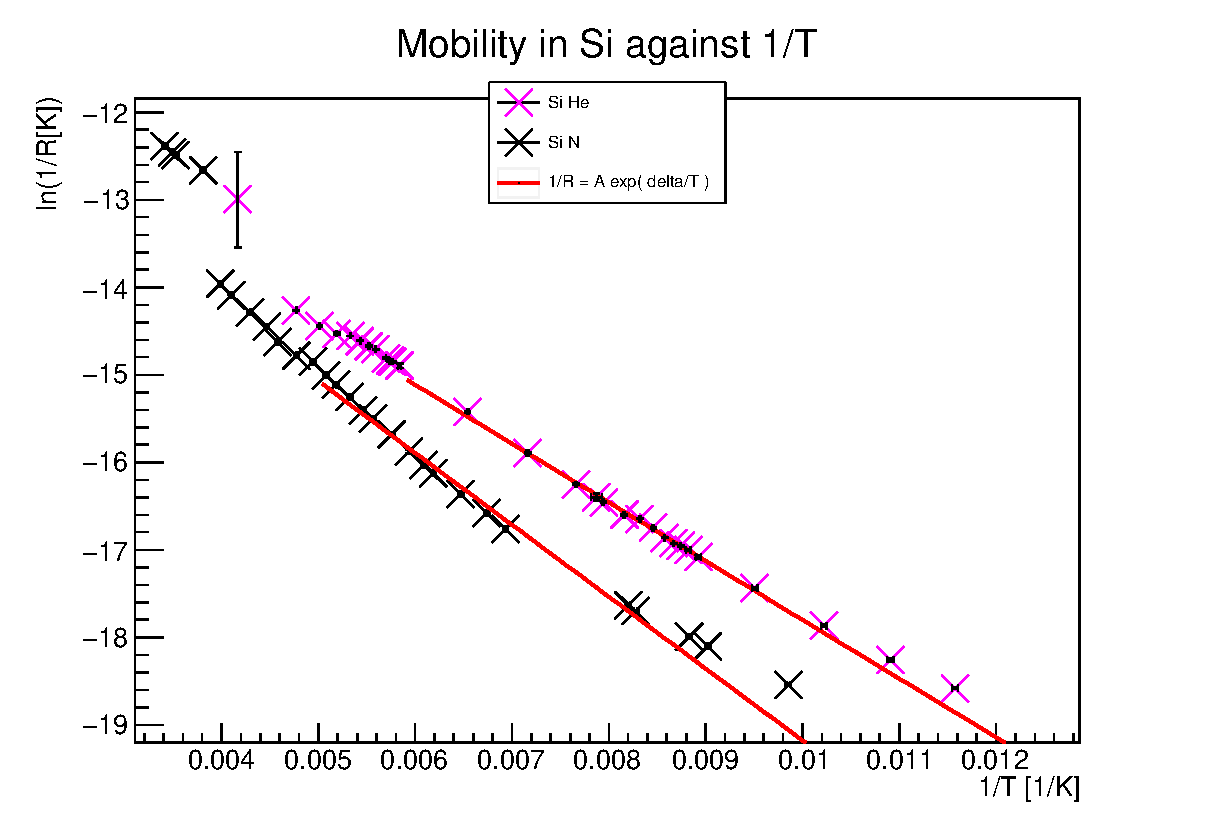
\includegraphics[width=\textwidth]{Graphen/Si_Tinv.eps}
    \caption{Fit for calculating the difference  activation energy of the acceptor and the valence energy of silicon}
    \label{Si}
\end{figure}
To calculate $\Delta E$ a linear function is fitted to the logarithmic data of silicon. The fit and the data is shown in fig.(\ref{Si}). The computed parameters are:
\begin{table}[H]
    \centering
        \begin{tabular}{l|l|l|l}
         & $\delta$ [K] & $\log(A[R])$ & $\chi^2/N_{dof}$\\\hline
        He & -671.139 $\pm$ 2.577  & -11.087 $\pm$ 0.022 & 24.4 \\
        N & -821.079 $\pm$ 2.129  & -10.966 $\pm$  0.013 & 217.8 \\
        \end{tabular}
\end{table}
To get $\Delta E$, $\delta$ has to be multiplied by $-2 k_B$. The results are
\begin{equation*}
    \Delta E_{He} = (0.116 \pm -0.001)eV \mbox{ and } \Delta E_{N} = (0.142 \pm -0.001)eV
\end{equation*}
The magnitude of the results is realistic and they are relative close to each other. Again the error of the results is way too small, which is caused by the calibration with only two and three points. An exact theoretical value is not given, since the energy of the valence in silicon is dependent on a magnitude of different factors and the donor energy is unknown.

\section{Conclusion}
All in all the errors in the calculations are difficult to estimate, because of the calibration with only as much data points as needed to solve the equation system.
Because of that the measurements in helium and nitrogen diverge a lot and are not really comparable.
Nevertheless the results for the temperature dependencies for copper and tantalum are close to the expected values, although the quality of the measurement is not given because of the not estimable errors.
It is safe to say, that every result contains large systemic errors, which are hard to estimate, since the Errors from the calibration can not be quantified properly.
If results from both the platinum and carbon calibrations are present and disagreeing, one should prefer the results obtained via the platinum, since these are more accurate at such high temperatures.
\newpage

\section{Source of literature values}
\begin{enumerate}
    \item linear coefficient: \url{https://www.electronics-notes.com/articles/basic_concepts/resistance/resistance-resistivity-temperature-coefficient.php}
\end{enumerate}
    
\end{document}

    % \begin{wrapfigure}[13]{l}[0cm]{7cm}
    %    \fbox{\includegraphics[width=7cm]{Bilder/Aufbau1.jpeg}}
    %   \caption{}
    % \end{wrapfigure}

    %\begin{table}[H]
    %\caption{}
    %    \begin{tabular}{|l|l|}
    %        \hline
    %        \\\hline
    %    \end{tabular}
    %\end{table}
    
    %\begin{figure}[H]
    %   \centering
    %    \includegraphics[width=\textwidth]{Graphen/Pendel_B_Roh.eps}
    %    \caption{Rohdaten von Pende} B mit markierten Nulldurchgängen und Auswertungsbereichl
    %    \label{fig:my_label}
    %\end{figure}
    
    %\begin{wraptable}[8]{l}[0.5cm]{5cm}
    %    \caption{Parameter der lin. Reg.}
    %    \begin{tabular}{|l|l|l|}
    %        \hline

    %       \hline
    %    \end{tabular}
    %\end{wraptable}
    
    %\begin{figure}
    %\begin{minipage}{0.5\textwidth}
    
    %\end{minipage}
    %\begin{minipage}{0.5\textwidth}
        %\captionof{figure}{Caption einzelne Bilder}
    %\end{minipage}
    %\caption{gesamte Bildunterschrift}
    %\label{}
\end{figure}